\documentclass[11pt]{article}
\usepackage[scaled=0.92]{helvet}
\usepackage{geometry}
\geometry{letterpaper,tmargin=1in,bmargin=1in,lmargin=1in,rmargin=1in}
\usepackage[parfill]{parskip} % Activate to begin paragraphs with an empty line rather than an indent %\usepackage{graphicx}
\usepackage{amsmath,amssymb, mathrsfs,  mathtools, dsfont}
\usepackage{tabularx}
\usepackage{tikz-cd}
\usepackage[font=footnotesize,labelfont=bf]{caption}
\usepackage{graphicx}
\usepackage{xcolor}
%\usepackage[linkbordercolor ={1 1 1} ]{hyperref}
%\usepackage[sf]{titlesec}
\usepackage{natbib}
\usepackage{../../Tianpei_Report}

%\usepackage{appendix}
%\usepackage{algorithm}
%\usepackage{algorithmic}

%\renewcommand{\algorithmicrequire}{\textbf{Input:}}
%\renewcommand{\algorithmicensure}{\textbf{Output:}}



\begin{document}
\title{Lecture 16: Geodesics}
\author{ Tianpei Xie}
\date{Nov. 4th., 2022}
\maketitle
\tableofcontents
\newpage
\section{Vector and Tensor Fields Along Curves}
\subsection{Definition}
\begin{itemize}
\item \begin{definition}
Let $M$ be a smooth manifold with or without boundary. Given a smooth curve $\gamma: I \rightarrow M$, \underline{\emph{\textbf{a vector field along $\gamma$}}} is a \emph{continuous} map $V: I \rightarrow TM$ such that $V(t) \in T_{\gamma(t)}M$ for every $t \in I$; it is \emph{\textbf{a smooth vector field along $\gamma$}} if it is \emph{smooth} as a map from $I$ to $TM$. 

We let $\frX(\gamma)$ denote \emph{\textbf{the set of all smooth vector fields along $\gamma$}}. It is a \emph{real vector space} under pointwise vector addition and multiplication by constants, and it is a module over $\cC^{\infty}(I)$ with multiplication defined pointwise:
\begin{align*}
(fX)(t) &= f(t)X(t).
\end{align*}
\end{definition}

\item \begin{example} (\emph{\textbf{The Velocity Vector Field}})\\
The most obvious example of \emph{a vector field along a smooth curve} $\gamma$ is the curve's \emph{\textbf{velocity}}: $\gamma'(t) \in T_{\gamma(t)}M$ for each $t$, and its coordinate expression 
\begin{align*}
\gamma'(t) &= \dot{\gamma}^i(t)\partdiff{}{x^i}
\end{align*} shows that it is \emph{\textbf{smooth}}. 
\end{example}

\item \begin{example} (\emph{\textbf{The Normal Vector Field}})\\
If $\gamma$ is a curve in $\bR^2$, let $N(t) = R\gamma'(t),$ where $R$ is \emph{\textbf{counterclockwise rotation}} by $\pi/2$, so $N(t)$ is \emph{\textbf{normal}} to $\gamma'(t)$. In standard coordinates, 
\begin{align*}
N(t) &= -\dot{\gamma}^2(t)\partdiff{}{x^1} + \dot{\gamma}^1(t)\partdiff{}{x^2},
\end{align*}
so \emph{\textbf{$N$ is a smooth vector field along $\gamma$}}.
\end{example}

\begin{figure}
\begin{minipage}[htb]{1\linewidth}
  \centering
  \centerline{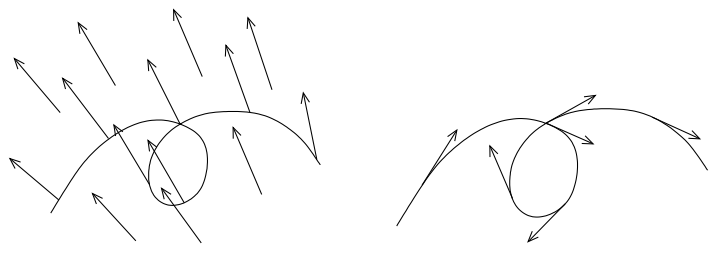
\includegraphics[scale = 0.5]{extendible_vector_field.png}}
\end{minipage}
\caption{\footnotesize{\textbf{An extendible vector field (Left) vs a non-extendible vector field \citep{lee2018introduction}}}}
\label{fig: extendible_vector_field}
\end{figure}


\item \begin{remark} (\emph{\textbf{Construction of A Smooth Vector Field Along the Curve}})\\
Suppose $\gamma: I \rightarrow M$ is a smooth curve and $\widetilde{V} \in \frX(M)$ is a smooth vector field on an open subset of $M$ containing the image of $\gamma$. The smooth vector field along the curve $\gamma$, $V = \widetilde{V} \circ \gamma$:
\begin{align*}
V(t) &= \widetilde{V}_{\gamma(t)} \in T_{\gamma(t)}M.
\end{align*} A smooth vector field along $\gamma$ is said to be \emph{\textbf{extendible}} if there \emph{exists} a smooth vector field $\widetilde{V}$ on
a neighborhood of the image of $\gamma$ that is related to $V$ in this way. 

\emph{\textbf{Not every vector field along a curve need be extendible}}; for example, if $\gamma(t_1) = \gamma(t_2)$ but $\gamma'(t_1) \neq \gamma'(t_2)$ (Fig. \ref{fig: extendible_vector_field}), then $\gamma'$ is not extendible. 
\end{remark}

\item \begin{definition}
More generally, \underline{\emph{\textbf{a tensor field along $\gamma$}}} is a \emph{continuous} map $\sigma$ from $I$ to some tensor bundle $T^{(k,l)}TM$ such that $\sigma(t) \in T^{(k,l)}T_{\gamma(t)}M$ for each $t \in I$. 

It is a \emph{\textbf{smooth tensor field along $\gamma$}} if it is \emph{smooth} as a map from $I$ to $T^{(k,l)}TM$, and it is \emph{\textbf{extendible}} if there is a smooth tensor field $\widetilde{\sigma}$ on a neighborhood of $\gamma(I)$ such that $\widetilde{\sigma} = \sigma \circ \gamma$.
\end{definition}
\end{itemize}
\subsection{Covariant Derivatives Along Curves}
\begin{itemize}
\item \begin{theorem} (\textbf{Covariant Derivative Along a Curve}). \\
Let $M$ be a smooth manifold with or without boundary and let $\nabla$ be a connection in $TM$. For each smooth curve $\gamma: I \rightarrow M$, the \textbf{connection} determines \textbf{a unique operator} 
\begin{align*}
D_t: \frX(\gamma) \rightarrow \frX(\gamma)
\end{align*} called \underline{\textbf{the covariant derivative along $\gamma$}}, satisfying the following properties:
\begin{enumerate}
\item (\textbf{Linearity over $\bR$}):
\begin{align*}
D_t\paren{a\,V + b\,W} &= a\,D_t(V) + b\,D_t(W), \quad \text{ for }a,b \in \bR.
\end{align*}
\item (\textbf{Product Rule}):
\begin{align*}
D_t(f\,V) &= f'\,V + f D_t(V), \quad \text{ for }f \in \cC^{\infty}(I).
\end{align*}
\item If $V \in \frX(\gamma)$ is \textbf{extendible}, then for every extension $\widetilde{V}$ of $V$,
\begin{align*}
D_t(V(t)) &= \conn{\gamma'(t)}{\widetilde{V}}.
\end{align*}
\end{enumerate} There is \textbf{an analogous operator} on the space of \textbf{smooth tensor fields} of any type along $\gamma$.
\end{theorem}


\item \begin{remark} (\emph{\textbf{Coordinate Representation for Covariant Derivatives Along a Curve}})\\
Choose smooth coordinates $(x^i)$ for $M$ in a neighborhood of $\gamma(t_0)$, and write
\begin{align*}
V(t) &=  V^{i}(t) \partdiff{}{x^i}\Bigr|_{\gamma(t)}
\end{align*} for $t$ near $t_0$, where $V^1 \xdotx{,} V^n$ are \emph{smooth real-valued functions} defined on some neighborhood of $t_0$ in $I$. By the properties of $D_t$, since each $\partdiff{}{x^i}$ is extendible,
\begin{align}
D_t\paren{V_t} &= \dot{V}^i(t) \partdiff{}{x^i}\Bigr|_{\gamma(t)} + V^i(t)\, \conn{\gamma'(t)}{\partdiff{}{x^i}\Bigr|_{\gamma(t)}} \nonumber\\
&= \paren{\dot{V}^k(t)  + \dot{\gamma}^{i}(t)V^j(t)\,\Gamma_{i,j}^{k}(\gamma(t))}\partdiff{}{x^k}\Bigr|_{\gamma(t)} \label{eqn: covariant_derivative_along_curve_represent}
\end{align}
\end{remark}

\item \begin{proposition}
Let $M$ be a smooth manifold with or without boundary, let $\nabla$ be a connection in $TM$, and let $p \in M$ and $v \in T_{p}M$. Suppose $Y$ and $\widetilde{Y}$ are two smooth vector fields that \textbf{agree} at points in the image of some smooth curve $\gamma: I \rightarrow M$ such that  $\gamma(t_0) = p$ and $\gamma'(t_0) = v$. Then $\conn{v}{Y} = \conn{v}{\widetilde{Y}}$.
\end{proposition}
\end{itemize}

\section{Geodesics}
\begin{itemize}
\item 
\begin{definition}
Let $M$ be a smooth manifold with or without boundary and let $\nabla$ be a connection in $TM$. For every smooth curve $\gamma: I \rightarrow M$, we define the \underline{\emph{\textbf{acceleration}}} of $\gamma$ to be \emph{\textbf{the vector field $D_t(\gamma')$ along $\gamma$}}.
\end{definition}

\item \begin{definition}
A smooth curve $\gamma$ is called a \underline{\emph{\textbf{geodesic}}} (\emph{\textbf{with respect to $\nabla$}}) if \emph{its acceleration is zero}: $D_t(\gamma'(t)) = 0$. 
\end{definition}

\item \begin{remark}
\emph{\textbf{Geodesic}} is the curve whose \emph{\textbf{tangential acceleration}} is \emph{\textbf{zero}}. From \emph{the connection $\nabla$ point of view}, it specify both the directional vector field and the target vector field equal to $\gamma'(t)$. That is, the \emph{tangential acceleration along a curve} $\gamma$ is 
\begin{align*}
\conn{\gamma'(t)}{\gamma'(t)}.
\end{align*}
\end{remark}

\item \begin{remark} (\emph{\textbf{The Ordinary Differential Equations for the Geodesic}})\\
In terms of smooth coordinates $(x^i)$, if we write the component functions of $\gamma$ as $\gamma(t) = (x^1(t) \xdotx{,} x^n(t))$. From \eqref{eqn: covariant_derivative_along_curve_represent} and  $D_t\paren{\gamma'(t)}$, we have a set of ordinary differential equations called \underline{\emph{\textbf{the geodesic equations}}}:
\begin{align}
\ddot{x}^k(t)  + \dot{x}^{i}(t)\dot{x}^j(t)\,\Gamma_{i,j}^{k}(x(t)) = 0, \quad k=1,\ldots, n \label{eqn: geodesic_equation}.
\end{align} where $x(t) := (x^1(t) \xdotx{,} x^n(t))$. A (parameterized) curve $\gamma$ is a geodesic \emph{\textbf{if and only if}} its component functions satiesfy \emph{the geodesic equations}. Note that \eqref{eqn: geodesic_equation} is \emph{\textbf{a set of \underline{second-order} \underline{nonlinear ODEs}}}.
\end{remark}

\begin{figure}
\begin{minipage}[htb]{1\linewidth}
  \centering
  \centerline{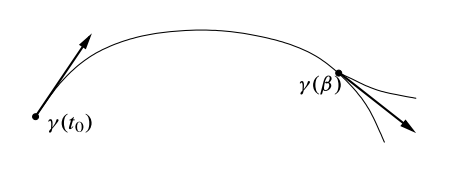
\includegraphics[scale = 0.5]{uniqueness_geodesics.png}}
\end{minipage}
\caption{\footnotesize{\textbf{The uniqueness of a geodesic \citep{lee2018introduction}}}}
\label{fig: uniqueness_geodesics}
\end{figure}


\item \begin{theorem}(\textbf{Existence and Uniqueness of Geodesics}). \citep{lee2018introduction} \\
Let $M$ be a smooth manifold and $\nabla$ a connection in $TM$. For every $p \in M$, $w \in T_{p}M$, and $t_0 \in \bR$, there \textbf{exist} an open interval $I \subseteq \bR$ containing $t_0$ and a \textbf{geodesic} $\gamma: I \rightarrow M$  satisfying $\gamma(t_0) = p$ and $\gamma'(t_0) = w$. Any two such geodesics \textbf{agree} on their common domain.
\end{theorem}

\item \begin{remark}
From the geodesic equation, we see that \emph{\textbf{the only parameters} of the ODE that determines the geodesic is \textbf{the cooefficients of the connection} $\{\Gamma_{i,j}^{k}\}$}. That is, \emph{the geodesic} is solely determined by \emph{the connection $\nabla$}. Thus we also call it a \emph{\textbf{$\nabla$-geodesic}}.
\end{remark}

\item \begin{remark} The \emph{\textbf{geodesic equation} under the initial boundary condition} can be written in the following form:
\begin{align}
\dot{x}^k(t) &= v^{k}(t) \\
\dot{v}^k(t) &= - v^{i}(t)v^j(t)\,\Gamma_{i,j}^{k}(x(t)) \label{eqn: geodesic_equation_first_order}
\end{align} Treating $(x^1 \xdotx{,} x^n, v^1 \xdotx{,} v^n)$ as coordinates on $U \times \bR^n$, we can recognize \eqref{eqn: geodesic_equation_first_order} as the equations for the \textbf{\emph{flow}} of \textbf{\emph{the vector field}} $G \in \frX(U \times \bR^n)$ given by
\begin{align}
G_{(x, v)} &= v^k\partdiff{}{x^k}\Bigr|_{(x, v)} - v^{i}v^j\,\Gamma_{i,j}^{k}(x)\partdiff{}{v^k}\Bigr|_{(x, v)}.
\end{align} The importance of $G$ stems from the fact that it actually defines \emph{\textbf{a global vector field on the total space of $TM$}}, called \underline{\emph{\textbf{the geodesic vector field}}}. It can be verified that the components of $G$ under a change of coordinates \emph{take the same form} in \emph{every coordinate chart}.

Note that $G$ acts on a function $f \in \cC^{\infty}(U \times \bR^n)$ as
\begin{align}
Gf(p, v) &= \frac{d}{dt}\Bigr|_{t=0}f(\gamma_v(t), \gamma_v'(t)). \label{eqn: geodesic_vector_field_act_function}
\end{align}
\end{remark}

\item \begin{definition}
A geodesic $\gamma: I \rightarrow M$  is said to be \emph{\textbf{maximal}} if it \emph{cannot be extended} to a geodesic on a \emph{larger interval}, that is, if there does not exist a geodesic $\widetilde{\gamma}: \widetilde{I} \rightarrow M$ defined on an interval $\widetilde{I}$ properly containing $I$ and satisfying $\widetilde{\gamma}|_{I} = \gamma$. 

\emph{A \textbf{geodesic segment}} is a geodesic whose domain is a \emph{\textbf{compact interval}}.
\end{definition}

\item \begin{corollary}
Let $M$ be a smooth manifold and let $\nabla$ be a connection in $TM$. For each $p \in M$ and $v \in T_{p}M$, there is a \textbf{unique maximal geodesic} $\gamma: I \rightarrow M$ with $\gamma(0) = p$ and $\gamma'(0) = v$, defined on some open interval $I$ containing $0$.
\end{corollary}

\item \begin{definition}
The \underline{\emph{\textbf{unique maximal geodesic}}} $\gamma$ with $\gamma(0) = p$ and $\gamma'(0) = v$ is often called simply \emph{\textbf{the geodesic with initial point $p$ and initial velocity $v$}}, and is denoted by $\gamma_v$. (Note that we can always find $p = \pi(v)$ where $\pi: TM \rightarrow M$ is the natural projection.)
\end{definition}
\end{itemize}

\section{Parallel Transport}
\begin{itemize}
\item \begin{definition}
Let $M$ be a smooth manifold and let $\nabla$ be a connection in $TM$. \emph{A smooth vector or tensor field $V$ along a smooth curve} $\gamma$ is said to be \emph{\textbf{parallel along} $\gamma$ (with respect to $\nabla$)} if $D_t(V) \equiv 0$.
\end{definition}

\begin{figure}
\begin{minipage}[htb]{1\linewidth}
  \centering
  \centerline{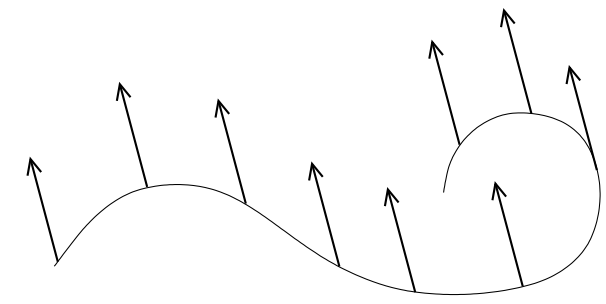
\includegraphics[scale = 0.45]{parallel_transport_along_curve.png}}
\end{minipage}
\caption{\footnotesize{\textbf{The parallel transport of a vector field along a curve \citep{lee2018introduction}}}}
\label{fig: parallel_transport_along_curve}
\end{figure}

\item \begin{remark}
A \emph{geodesic} can be characterized as a curve whose \emph{\textbf{velocity vector field is parallel along the curve}}.
\end{remark}

\item \begin{remark} (\emph{\textbf{Coordinate Representation of Vector Field Parallel Along a Curve}})\\
Given a smooth curve $\gamma$ with a local coordinate representation $\gamma(t) = (\gamma^1(t) \xdotx{,} \gamma^n(t))$, formula \eqref{eqn: covariant_derivative_along_curve_represent} shows that a vector field $V$ is parallel along $\gamma$ if and only if
\begin{align}
\dot{V}^k(t)  + \dot{\gamma}^{i}(t)V^j(t)\,\Gamma_{i,j}^{k}(\gamma(t)) = 0, \quad k=1,\xdotx{,} n \label{eqn: vector_field_parallel_along_curve_represent}
\end{align} This is a set of \emph{\textbf{linear ordinary differential equations}} with respect to $(V^1(t) \xdotx{,} V^n(t))$.
\end{remark}

\item For linear ODEs, we have stronger results:
\begin{theorem} (\textbf{Existence, Uniqueness, and Smoothness for Linear ODEs}). \citep{lee2018introduction} \\
Let $I \subseteq R$ be an open interval, and for $1 \le j, k \le n$, let $A_j^k: I \rightarrow \bR$ be smooth functions. For all $t_0 \in I$ and every initial vector $(c^1 \xdotx{,} c^n) \in \bR^n$, the \textbf{linear initial value problem}
\begin{align}
\dot{V}^k(t) &= A_j^{k}(t)\, V^j(t),  \label{eqn: linear_ode} \\
V^k(t_0) &= c^k, \nonumber
\end{align} has a \textbf{unique smooth solution} on \textbf{all} of $I$, and the solution depends \textbf{smoothly} on $(t, c) \in I \times \bR^n$.
\end{theorem}

\item \begin{theorem} (\textbf{Existence and Uniqueness of Parallel Transport}). \\
Suppose $M$ is a smooth manifold with or without boundary, and $\nabla$ is a connection in $TM$. Given a smooth curve $\gamma: I \rightarrow M$, $t_0 \in I$, and a vector $v \in T_{\gamma(t_0)}M$ or tensor $v \in T^{(k,l)}T_{\gamma(t_0)}M$, there exists a \textbf{unique parallel vector or tensor field $V$} along $\gamma$ such that $V(t_0) = v$.
\end{theorem}

\item \begin{remark}
Compare to results for geodesic, there is no need for definition similar to \emph{the maximal geodesic} since \emph{\textbf{the solution for parallel transport is global on all $I$}}.
\end{remark}

\item \begin{remark}
\emph{The vector or tensor field} whose existence and uniqueness are proved in Theorem aboive is called \emph{\textbf{the parallel transport of $v$ along $\gamma$}}.
\end{remark}

\item \begin{definition}
For each $t_0, t_1 \in I$, we define a map 
\begin{align}
P^{\gamma}_{t_0, t_1}: T_{\gamma(t_0)}M \rightarrow T_{\gamma(t_1)}M,  \label{eqn: parallel_transport_map}
\end{align} called \underline{\emph{\textbf{the parallel transport map}}}, by setting 
\begin{align*}
P^{\gamma}_{t_0, t_1}(v) &= V(t_1), \quad \forall v \in T_{\gamma(t_0)}M
\end{align*} where \emph{$V$ is the \textbf{parallel transport} of $v$ along $\gamma$}. 

This map is \emph{\textbf{linear}}, because \emph{the equation of parallelism is linear}. It is in fact an \emph{\textbf{isomorphism}}, because $P^{\gamma}_{t_1, t_0}$ is an \emph{\textbf{inverse}} for it.
\end{definition}

\item \begin{definition}
Given an \emph{\textbf{admissible curve}} $\gamma: [a, b] \rightarrow M$, a map $V: [a, b] \rightarrow TM$ such that $V(t) \in T_{\gamma(t)}M$ for each $t$ is called \emph{\textbf{a piecewise smooth vector field along $\gamma$}} if $V$ is continuous and there is an \emph{admissible partition} $(a_0 \xdotx{,} a_k)$ for $\gamma$ such that $V$ is smooth on each subinterval $[a_{i-1}, a_i]$. We will call any such partition \emph{\textbf{an admissible partition for $V$}}. \emph{A piecewise smooth vector field V along $\gamma$} is said to be \emph{\textbf{parallel}} along $\gamma$ if $D_t(V) = 0$ wherever $V$ is smooth.
\end{definition}

\item \begin{corollary} (\textbf{Parallel Transport Along Piecewise Smooth Curves}). \\
Suppose $M$ is a smooth manifold with or without boundary, and $\nabla$ is a connection in $TM$. Given an admissible curve $\gamma: [a, b] \rightarrow M$ and a vector $v \in T_{\gamma(t_0)}M$ or tensor $v \in T^{(k,l)}T_{\gamma(t_0)}M$, there exists a \textbf{unique piecewise smooth} \textbf{parallel} vector or tensor field $V$ along $\gamma$ such that $V(a) = v$, and $V$ is smooth wherever $\gamma$ is.
\end{corollary}

\item \begin{remark} (\emph{\textbf{Parallel Frames Along a Curve}})\\
Given any basis $(b_1 \xdotx{,} b_n)$ for $T_{\gamma(t_0)}M$, we can \emph{\textbf{parallel transport the vectors $b_i$ along $\gamma$}}, thus obtaining an $n$-tuple of \emph{parallel vector fields} $(E_1 \xdotx{,} E_n)$  along $\gamma$. Because each parallel transport map is an \emph{isomorphism}, \emph{\textbf{the vectors $(E_i(t))$ form a basis for $T_{\gamma(t)}M$ at each point $\gamma(t)$}}. Such an $n$-tuple of vector fields along $\gamma$ is called \emph{\textbf{a
parallel frame along $\gamma$}}.

Every smooth (or piecewise smooth) vector field along $\gamma$ can be expressed in terms of such a frame as 
\begin{align*}
V(t) = V^i(t)\, E_i(t),
\end{align*} and then the properties of covariant derivatives along curves, together with the fact that the $E_i$'s are parallel,
imply
\begin{align}
D_t(V_t) &= \dot{V}^i(t)\, E_i(t)  \label{eqn: parallel_transport_basis_vector_fields}
\end{align} wherever $V$ and $\gamma$ are smooth. This means that \emph{a vector field is \textbf{parallel} along $\gamma$} \emph{if and only} if \emph{\textbf{its component functions with respect to the frame $(E_i)$ are constants}}.
\end{remark}

\item \begin{theorem} (\textbf{Parallel Transport Determines Covariant Differentiation}). \citep{lee2018introduction}\\
Let $M$ be a smooth manifold with or without boundary, and let $\nabla$ be a connection in $TM$. Suppose $\gamma: I \rightarrow M$ is a smooth curve and $V$ is a smooth vector field along $\gamma$. For each $t_0 \in I$,
\begin{align}
D_t V(t_0) &=\lim_{\Delta t \rightarrow 0}\frac{P^{\gamma}_{(t_0+\Delta t), t_0}(V(t_0+\Delta t))  - V(t_0)}{\Delta t} \label{eqn: covariant_derivatives_from_parallel_transport}
\end{align}
\end{theorem}

\item \begin{corollary} (\textbf{Parallel Transport Determines the Connection}). \citep{lee2018introduction} \\
Let $M$ be a smooth manifold with or without boundary, and let  $\nabla$ be a connection in $TM$. Suppose $X$ and $Y$ are smooth vector fields on $M$. For every $p \in M$,
\begin{align}
\conn{X}{Y}\bigr|_{p}&=\lim_{t \rightarrow 0}\frac{P^{\gamma}_{t, 0}(Y_{\gamma(t)})  - Y_p}{t}, \label{eqn: connection_from_parallel_transport}
\end{align} where $\gamma: I \rightarrow M$ is any smooth curve such that $\gamma(0) = p$ and $\gamma'(0) = X_p$.
\end{corollary}

\item \begin{remark}
See similarity between \eqref{eqn: connection_from_parallel_transport} and the definition of Lie derivatives:
\begin{align*}
\paren{\mathscr{L}_{X}\,Y}_{p}  &= \lim_{t\rightarrow 0}\frac{ d(\theta_{-t})_{\theta_{t}(p)}\paren{Y_{\theta_t(p)}}   - Y_{p}}{t},
\end{align*} where $\theta$ is the \emph{\textbf{flow of $X$}} in the neighborhood of $p$ such that $\theta_0(p) = p$, $(\theta^{(p)})'(0) = X_p$.
\end{remark}

\item \begin{remark}
A smooth vector or tensor field on $M$ is said to be \emph{\textbf{parallel}} \emph{(with respect to $\nabla$)} if it is \emph{parallel along \textbf{every smooth curve} in $M$}. 
\end{remark}

\item \begin{proposition}
Suppose $M$ is a smooth manifold with or without boundary, $\nabla$ is a connection in $TM$, and $A$ is a \textbf{smooth vector or tensor field} on $M$. Then $A$ is
parallel on $M$ if and only if $\nabla A \equiv 0$.
\end{proposition}

\item \begin{remark}
It is always possible to extend a vector at a point to a parallel vector field along any given curve. However, it may not be possible in general to extend it to a \emph{\textbf{parallel vector field}} on an open subset of the manifold. The impossibility of finding such extensions is intimately connected with the phenomenon of \emph{\textbf{curvature}}.
\end{remark}
\end{itemize}

\section{Pullback Connections}
\begin{itemize}
\item \begin{remark}
Like vector fields, connections in the tangent bundle \textbf{cannot} be either pushed forward or pulled back by arbitrary smooth maps.
\end{remark}

\item 
\begin{lemma} (\textbf{Pullback Connections}). \citep{lee2018introduction} \\
Suppose $M$ and $\widetilde{M}$ are smooth manifolds with or without boundary. If $\widetilde{\nabla}$ is a connection in $T\widetilde{M}$ and  $\varphi: M \rightarrow \widetilde{M}$ is a \underline{\textbf{diffeomorphism}}, then the map $\varphi^{*}\widetilde{\nabla}:  \frX(M) \times \frX(M) \rightarrow \frX(M)$ defined by
\begin{align}
(\varphi^{*}\widetilde{\nabla})_{X}Y&= (\varphi^{-1})_{*}\paren{\widetilde{\nabla}_{\varphi_{*}X}{(\varphi_{*}Y)}} \label{eqn: pullback_connections}
\end{align} is a connection in $TM$, called \underline{\textbf{the pullback of $\widetilde{\nabla}$ by $\varphi$}}. Here $\varphi_{*}X, \varphi_{*}Y$ are pushforward of $X$ and $Y$ by $\varphi$. $(\varphi^{-1})_{*}(Z)$ is the pushforward of $Z$ by $\varphi^{-1}$.
\end{lemma}

\item The next proposition shows that various important concepts defined in terms of connections -- covariant derivatives along curves, parallel transport, and geodesics—
all behave as expected with respect to pullback connections.
\begin{proposition} (\textbf{Properties of Pullback Connections}).\\
Suppose $M$ and $\widetilde{M}$ are smooth manifolds with or without boundary, and $\varphi: M \rightarrow \widetilde{M}$ is a diffeomorphism.
Let $\widetilde{\nabla}$  be a connection in $T\widetilde{M}$ and let $\nabla = \varphi^{*}\widetilde{\nabla}$ be the \textbf{pullback connection} in $TM$.
Suppose $\gamma: I \rightarrow M$  is a smooth curve.
\begin{enumerate}
\item $\varphi$ takes \textbf{covariant derivatives along curves to covariant derivatives along curves}: if $V$ is a smooth vector field along $\gamma$, then
\begin{align*}
d\varphi \circ D_t(V) &= \widetilde{D}_t(d\varphi \circ V),
\end{align*}
where $D_t$ is covariant differentiation along $\gamma$ with respect to $\nabla$, and $\widetilde{D}_t$ is
covariant differentiation along $\varphi \circ \gamma$ with respect to $\widetilde{\nabla}$.
\item $\varphi$ takes \textbf{geodesics to geodesics}: if $\gamma$ is a $\nabla$-geodesic in $M$, then $\varphi \circ \gamma$ is a
$\widetilde{\nabla}$-geodesic in $\widetilde{M}$.
\item $\varphi$ takes \textbf{parallel transport to parallel transport}: for every $t_0, t_1 \in I$,
\begin{align*}
d\varphi_{\gamma(t_1)} \circ P^{\gamma}_{t_0, t_1} &= P^{\varphi \circ \gamma}_{t_0, t_1} \circ d\varphi_{\gamma(t_0)}.
\end{align*}

\end{enumerate}
\end{proposition}
\end{itemize}

\newpage
\bibliographystyle{plainnat}
\bibliography{book_reference.bib}
\end{document}